\documentclass[oribibl]{llncs}

\usepackage{amsmath,amssymb,graphicx,dsfont}

\newcommand{\mml}{\ensuremath{(\mu/\mu,\lambda)}}
\newcommand{\T}{\ensuremath{\mathrm{T}}}
\newcommand{\s}{\ensuremath{\mathbf{s}}}
\renewcommand{\v}{\ensuremath{\mathbf{v}}}
\newcommand{\w}{\ensuremath{\mathbf{w}}}
\newcommand{\x}{\ensuremath{\mathbf{x}}}
\newcommand{\y}{\ensuremath{\mathbf{y}}}
\newcommand{\z}{\ensuremath{\mathbf{z}}}
\newcommand{\avg}{\ensuremath{\text{(avg)}}}
\newcommand{\dR}{\ensuremath{\mathbb{R}}}
\DeclareMathOperator{\sgn}{sgn}
\newcommand{\cmml}{\ensuremath{c_{\mu/\mu,\lambda}}}
\setlength{\tabcolsep}{4pt}

%\renewcommand{\floatpagefraction}{.9}
%\renewcommand{\topfraction}{.9}

%\setlength{\pdfpagewidth}{8.5in}
%\setlength{\pdfpageheight}{11in}


\title{An Active-Set Evolution Strategy for Optimization with Known Constraints}

\author{Dirk V.~Arnold}
\institute{Faculty of Computer Science, Dalhousie University\\
       Halifax, Nova Scotia, Canada B3H 4R2\\
       \email{dirk@cs.dal.ca}}


\begin{document}

\maketitle

\begin{abstract}


We propose an evolutionary approach to constrained optimization where the objective function is considered a black box, but the constraint functions are assumed to be known. The approach can be considered a stochastic active-set method. It labels constraints as either active or inactive and projects candidate solutions onto the subspace of the feasible region that is implied by rendering active inequality constraints equalities. We implement the approach in a $(1+1)$-ES and evaluate its performance using a commonly used set of test problems.
\end{abstract}


\section{Introduction}

Evolutionary algorithms are stochastic black box optimization strategies. They are commonly used in connection with optimization problems that do not admit a convenient mathematical representation of the objective, or if gradient estimates can be obtained only at a high cost or are necessarily inaccurate. Examples include scenarios where the evaluation of the quality of a candidate solution requires running a simulation model. In the context of constrained optimization with evolutionary algorithms, the constraint functions are often considered as black boxes as well. However, in many cases, including the case of bound constraints, it is not uncommon that the constraint functions are known and relatively inexpensive to evaluate. The objective of this paper is to develop a simple evolutionary algorithm for constrained optimization with known constraints.

Active-set methods are a common approach to solving constrained optimization problems~\cite{NW06}. They maintain a set of active inequality constraints and perform optimization in the subspace of the feasible region that is implied by rendering the active inequality constraints equalities. The algorithm we introduce in this paper can be considered a stochastic active-set approach implemented in a $(1+1)$-ES\footnote{See Hansen et al.~\cite{hansen15} for an introduction to evolution strategy terminology.}. The step size of the $(1+1)$-ES is commonly controlled using the 1/5th rule~\cite{rechenberg73}. That rule can fail in the presence of small constraint angles (i.e., small angles between the gradient of the objective function and the normal vector of the constraint function) in cases as simple as a linear objective with a single linear constraint~\cite{schwefel81,arnold08}. Small constraint angles result in low success rates and thus a systematic reduction of the step size. Projection of infeasible candidate solutions onto the feasible region in connection with an active-set approach can potentially circumvent unwarranted decreases of the step size.

The remainder of this paper is organized as follows. In Section~\ref{sec2} we outline the class of optimization problems we strive to solve, formalize notation, and propose an active-set $(1+1)$-ES for optimization with known constraints. In Section~\ref{sec3}, that algorithm is applied to commonly used test problems and its performance is discussed. Section~\ref{sec4} concludes.


\section{\label{sec2}Problem and Algorithm}

%We introduce notational conventions and terminology in Section~\ref{sec2.1} and present an active-set $(1+1)$-ES in Section~\ref{sec2.2}.


%\subsection{\label{sec2.1}Problem and Terminology}

We consider the problem of minimizing objective function $f:\mathbb{R}^n\rightarrow\mathbb{R}$ subject to constraints
\begin{equation}\label{eq.constraints}
  \begin{split}
    g_i&(\x)\leq0\hspace{5mm}\text{for $i\in\{1,\dots,l\}$}\\
    h_j&(\x)=0\hspace{5mm}\text{for $j\in\{1,\dots,m\}$}\,.
  \end{split}
\end{equation}
The active set $\mathcal{A}(\x)$ of a (feasible) candidate solution~$\x$ is the set of indices of all those inequality constraints with $g_i(\x)=0$. Assuming a single globally optimal solution~$\x^*$ to the optimization problem, we refer to the active set~$\mathcal{A}(\x^*)$ of that solution as the optimal active set $\mathcal{A}^*$. We refer to the subspace of the search space where all equality constraints and active inequality constraints in $\mathcal{A}(\x)$ are satisfied as equalities as the reduced search space at~$\x$. We write $n^*$ for the dimension of the reduced search space at the optimal solution~$\x^*$.


%\subsection{\label{sec2.2}Algorithm}
 
Our active-set $(1+1)$-ES evolves a feasible candidate solution~$\x\in\mathbb{R}^n$ to the optimization problem at hand, adapting the step size~$\sigma\in\mathbb{R}_+$ using the 1/5th rule. Offspring candidate solutions are usually projected onto the reduced search space at the parent. However, with a certain probability the use of the active set is suspended, allowing to break out of the reduced search space. Adapting the step size of the algorithm only in those steps where the active inequalities are enforced as equalities prevents unwarranted decreases of the step size. A single iteration of the algorithm is described in Fig.~\ref{fig1}.

\begin{figure}[t]
  \fbox{\begin{minipage}{.98\linewidth}
    \hfill\parbox{.96\linewidth}{%
    \begin{enumerate}\renewcommand\itemsep{2mm}
      \item Compute the dimension $n'=n-\mathrm{rank}(N)$ of the reduced search space at~$\x$, where $N$ is the matrix whose columns are the normal vectors at~$\x$ of the equality constraints and the inequality constraints in $\mathcal{A}(\x)$.
      \item Repeat\vspace{2mm}
        \begin{enumerate}
          \item Generate standard normally distributed $\z\in\mathbb{R}^n$ and
	    let
	    \begin{displaymath}
	      \y=\x+\sigma\z\,.
	    \end{displaymath}
          \item If $n'=0$, let $\kappa$ be true. If $n'>0$, let $\kappa$ be true with probability $p$ and false otherwise.
          \item If $\kappa$ is true, project $\y$ onto the feasible region; otherwise, project $\y$ onto the intersection of the feasible region with the reduced search space at~$\x$.
        \end{enumerate}\vspace{2mm}
	until offspring candidate solution $\y\in\mathbb{R}^n$ is feasible.
      \item If $f(\y)<f(\x)$, then\vspace{2mm}
        \begin{enumerate}
	  \item Let
            \begin{displaymath}
              \x\gets\y\,.
            \end{displaymath}
	  \item If $\kappa$ is false, let
	    \begin{displaymath}
	      \sigma\gets\sigma2^{1/n'}\,.
	    \end{displaymath}
	\end{enumerate}\vspace{2mm}
        Otherwise, if $\kappa$ is false, let
        \begin{displaymath}
          \sigma\gets\sigma2^{-1/(4n')}\,.
        \end{displaymath}
    \end{enumerate}}\hspace{4mm}
    \end{minipage}}
  \caption{\label{fig1}Single iteration of the active-set $(1+1)$-ES.}
\end{figure}

Boolean flag~$\kappa$ determines whether or not the active set of~$\x$ is enforced for offspring candidate solution~$\y$. If $\kappa$ is false, then the search proceeds in the reduced search space. If it is true, then the inequality constraints active at the parental candidate solution will be enforced as inequalities rather than as equalities. If the dimension of the reduced search space at~$\x$ is zero, then there is no use in enforcing the active constraints as they would repeatedly yield the same solution, and $\kappa$ is thus set to true. Otherwise, the active inequality constraints are enforced as equality constraints with probability~$1-p$. Larger values of $p$ decrease the likelihood that the algorithm will spend unproductive time in non-optimal reduced subspaces. However, once the optimal active set~$\mathcal{A}^*$ has been found, smaller values of $p$ are useful as unproductive steps beyond the optimal reduced search space are avoided. We use $p=0.2$ throughout.

Projection of $\y$ onto the intersection of the feasible region with the reduced search space at~$\x$ is accomplished by minimizing function $d(\w)= \|\w-\y\|^2$ subject to constraints
\begin{align*}
  g_i(\w)&\leq0\hspace{5mm}\text{for $i\in\{1,\dots,l\}\setminus\mathcal{A}(\x)$}\\
  g_i(\w)&=0\hspace{5mm}\text{for $i\in\mathcal{A}(\x)$}\\
  h_j(\w)&=0\hspace{5mm}\text{for $j\in\{1,\dots,m\}$}\,.
\end{align*}
When the use of the active set is suspended, projection onto the feasible region is accomplished by minimizing that some function, but subject to the original set of constraints from Eq.~\eqref{eq.constraints}. Notice that minimization does not make use of the objective~$f$ of the original optimization problem and that thus the algorithm performs only a single evaluation of $f$ per iteration. Minimization of $d$ can be accomplished using any algorithm for constrained optimization. We use the active-set method implemented in \texttt{fmincon} in \textsl{Matlab}'s optimization toolbox. Step~2 involves a loop as minimization of $d$ may fail to yield a feasible solution.

\begin{figure}[t]
  \begin{minipage}{\linewidth}
    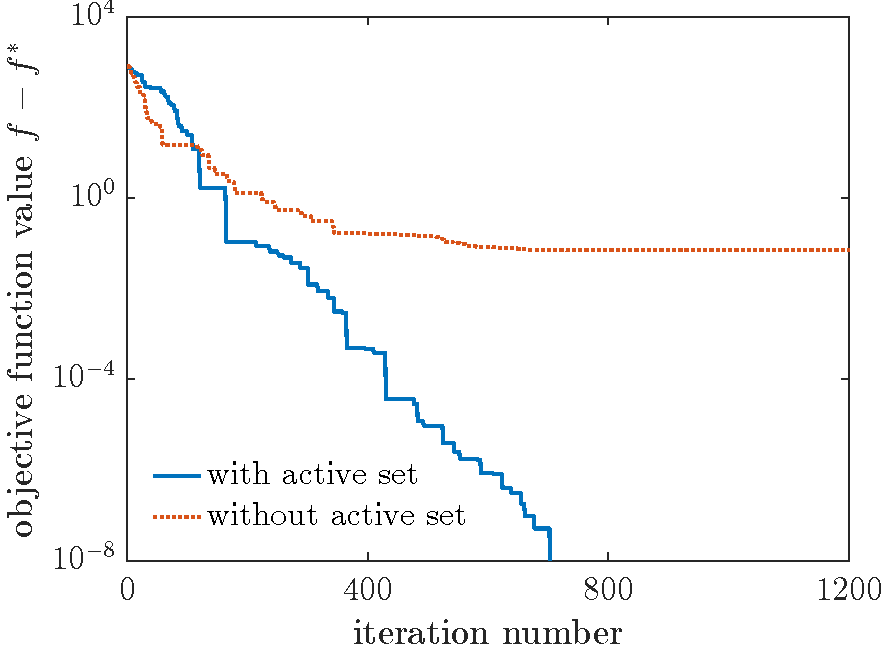
\includegraphics[width=.48\linewidth]{figures/sphere1}
    \hfill
    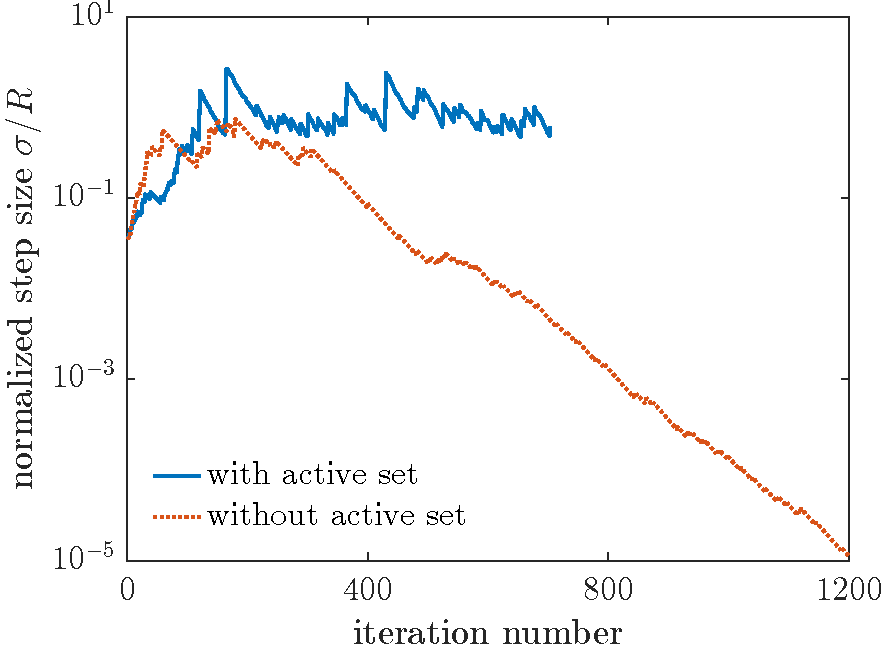
\includegraphics[width=.48\linewidth]{figures/sphere2}
  \end{minipage}
  \caption{\label{fig.sphere}Traces from runs of the active-set $(1+1)$-ES and a $(1+1)$-ES that projects infeasible candidate solutions onto the feasible region but does not enforce active inequalities as equalities applied to a $10$-dimensional sphere with five mutually orthogonal linear inequality constraints active at the optimal solution. Shown are the evolution of the difference between $f(\x)$ and the optimal objective function value $f^*$ and the step size $\sigma$ normalized by division by $R=\|\x-\x^*\|$.}
\end{figure}

The update of $\sigma$ in Step~3 of the algorithm employs the implementation of the 1/5th rule due to Kern et al.~\cite{kern04}. The step size is updated only in those iterations where the search proceeds in the reduced search space, thus avoiding the issue of systematically decreasing $\sigma$ when the use of the active set is suspended.

Throughout a run of the algorithm, we store the current active set. Constraints are added to the active set whenever a candidate solution is accepted for which those constraints are tight. Notice that it is straightforward from the output of \texttt{fmincon} to determine which constraints are tight by identifying those inequality constraints that have positive Lagrange multipliers. The active set is replaced in those iterations where a candidate solution replaces its parent that is generated with use of the active set suspended.
 
Figure~\ref{fig.sphere} illustrates the advantage of the active-set based approach over a $(1+1)$-ES that simply projects infeasible candidate solutions onto the feasible region, without enforcing active inequality constraints as equalities, and that updates the step size in every iteration. We have conducted 21 runs of both strategies for objective function $f(\x)=\x^\mathrm{T}\x$ with $n=10$ and constraints $\x^\mathrm{T}\mathbf{e}_i\geq1$ for $i\in\{1,\dots,5\}$, where $\mathbf{e}_i$ is the unit vector in the direction of the $i$th coordinate axis. All runs are initialized to start at $\x=(9,\dots,9)^\mathrm{T}$ and with step size $\sigma=1$. The active-set $(1+1)$-ES attained an objective function value within a factor of $(1+10^{-8})$ of the optimal objective function value $f^*=f(\x^*)$ in each of the runs; the run that required the median number of iterations is shown in the figure. It can be seen that the strategy converges linearly, and that after an initial increase, the step size~$\sigma$ is controlled to be approximately proportional to the distance~$R$ from the optimal solution~$\x^*$. Not shown, in the run depicted, the five constraints become active between the 66th and the 100th iteration and remain active until the algorithm terminates. Without the use of the active set, none of the 21 runs obtained a solution with an objective function value within a factor of $(1+10^{-8})$ of $f^*$ before terminating after 1,{}200 iterations. The corresponding trace shown in the figure is that of a random run. It can be seen that not enforcing active inequalities as equalities and updating $\sigma$ in every iteration eventually results in very small step sizes and slow progress.



\section{\label{sec3}Evaluation and Discussion}

We evaluate the active-set $(1+1)$-ES by applying it to the test problems \texttt{g01} through \texttt{g11} gathered by Michalewicz and Schoenauer~\cite{MS96} and summarized by Liang et al.~\cite{CEC06}. We initialize the parental candidate solution by uniformly randomly sampling a point in the bound constrained search space and then projecting it onto the feasible region using the same approach as described for offspring candidate solutions in Section~\ref{sec2}. The initial step size is set to $\sigma=0.2\min\{u_i-l_i\,|\,i=1,\dots,n\}$, where the $l_i$ and $u_i$ are the lower and upper bounds of the search space in dimension~$i$ for the respective problem. A run of the algorithm is terminated and considered a success if a candidate solution~$\x$ with an objective function value $f(\x)<(1+\epsilon)f^*$ is found, where $f^*$ is the objective function value of the optimal solution to the problem. It is considered unsuccessful if after 1,{}200 iterations (and thus as many evaluations of the objective function) no solution satisfying the termination criterion has been found. We refer to $\epsilon$ as the target accuracy.

\begin{table}[t]
  \caption{\label{tab.results}Test function properties and results.}
  \centering
  \begin{tabular}{lrrrrrrrrrrr}
    & \texttt{g01}
    & \texttt{g02} 
    & \texttt{g03} 
    & \texttt{g04} 
    & \texttt{g05} 
    & \texttt{g06} 
    & \texttt{g07} 
    & \texttt{g08} 
    & \texttt{g09} 
    & \texttt{g10} 
    & \texttt{g11}\\
    \hline
    dimension $n$
      & 13 & 20 & 10 & 5 & 4 & 2 & 10 & 2 & 7 & 8 & 2\\
    reduced dimension $n^*$
      &  0 & 19 &  9 & 0 & 1 & 0 &  4 & 2 & 5 & 2 & 1\\
    \hline
    success rate:\\
    \ \ \ \ $\epsilon=10^{-4}$
      & 1.0 & 0.0 & 1.0 & 1.0 & 1.0 & 1.0 & 0.98 & 0.52 & 1.0 & 1.0 & 1.0\\
    \ \ \ \ $\epsilon=10^{-8}$
      & 1.0 & 0.0 & 1.0 & 1.0 & 1.0 & 1.0 & 0.99 & 0.53 & 1.0 & 1.0 & 1.0\\
    \hline
    \multicolumn{10}{l}{median number of function evaluations:}\\
    \ \ \ \ $\epsilon=10^{-4}$
      & 49 & --- & 458 & 22 & 36 & 3 & 411 & 123 & 302 & 117 & 27\\
    \ \ \ \ $\epsilon=10^{-8}$
      & 46 & --- & 865 & 24 & 84 & 4 & 684 & 229 & 616 & 243 & 106\\
      \hline
  \end{tabular}
\end{table}

We have conducted 100 runs of the algorithm for each test problem and target accuracies $\epsilon\in\{10^{-4},10^{-8}\}$\footnote{The \texttt{ConstraintTolerance} parameter of \texttt{fmincon} is set to its default value of $10^{-6}$ for the runs with target accuracy~$\epsilon=10^{-4}$. For target accuracy $\epsilon=10^{-8}$ we used \texttt{ConstraintTolerance} $10^{-9} $ instead as some runs for problem \texttt{g03} terminate unsuccessfully if the default accuracy is used.}. Table~\ref{tab.results} summarizes the results. For eight of the eleven test problems, the globally optimal solution was found to the desired accuracy in all 100 runs conducted. The three exceptions are as follows:
\begin{itemize}
  \item For \texttt{g02} not a single run successfully located the globally optimal solution. Problem~\texttt{g02} has a very large number of local minima, and the search space is such that the likelihood of starting in the basin of attraction of the global optimum is near zero. A stochastic hill climber, such as the $(1+1)$-ES, will almost always converge toward a merely local minimum.
  \item A small number of unsuccessful runs are observed for problem \texttt{g07}, even though the problem is unimodal. The search space is ten-dimensional, with six inequality constraints active at the optimal solution. In some runs, the upper bound constraint for variable $x_8$ is included in the active set of the algorithm at some point during the run. The likelihood of escaping the point that is optimal for this active set in one of the steps where the use of the active set is suspended can be observed to be no higher than 5\% for a large range of values of the step size. It may thus take hundreds of iterations before the upper bound constraint is rendered inactive, and either reaching the iteration limit or the step size becoming so small that the limits of numerical accuracy are reached prevents successfully escaping the non-optimal reduced search space.
  \item Problem \texttt{g08} has four locally optimal solutions. No constraints are active at the globally optimal one of those. The $(1+1)$-ES converges to one of the merely locally optimal solutions with a likelihood of just under one half. Conducting multiple runs of the algorithm would allow locating the globally optimal solution with high probability.
\end{itemize}

\begin{figure}
  \begin{minipage}{\linewidth}
    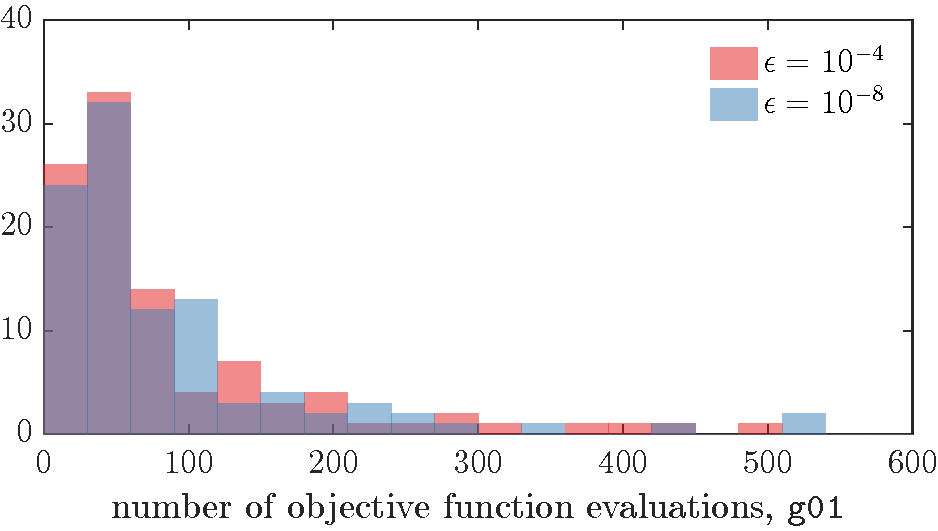
\includegraphics[width=.48\linewidth]{figures/hist01}
    \hfill
    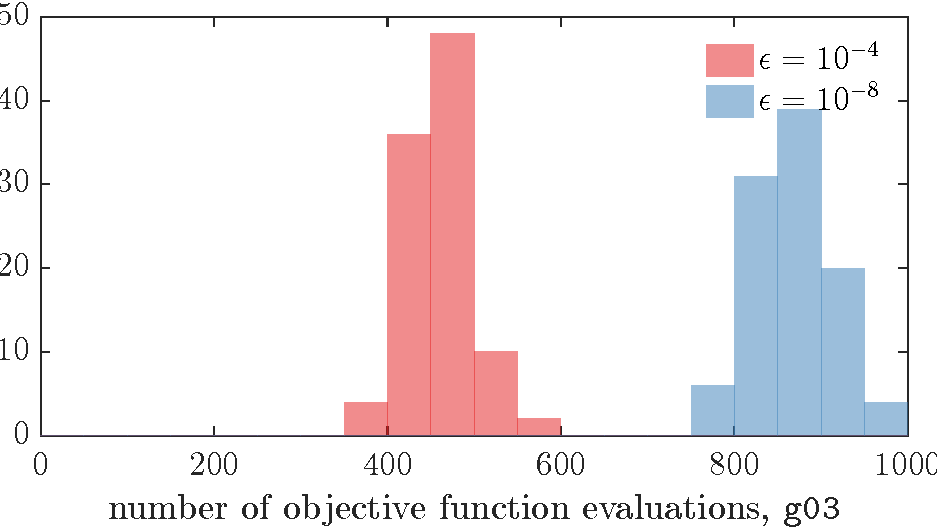
\includegraphics[width=.48\linewidth]{figures/hist03}
    
    \vspace{3.6mm}
    
    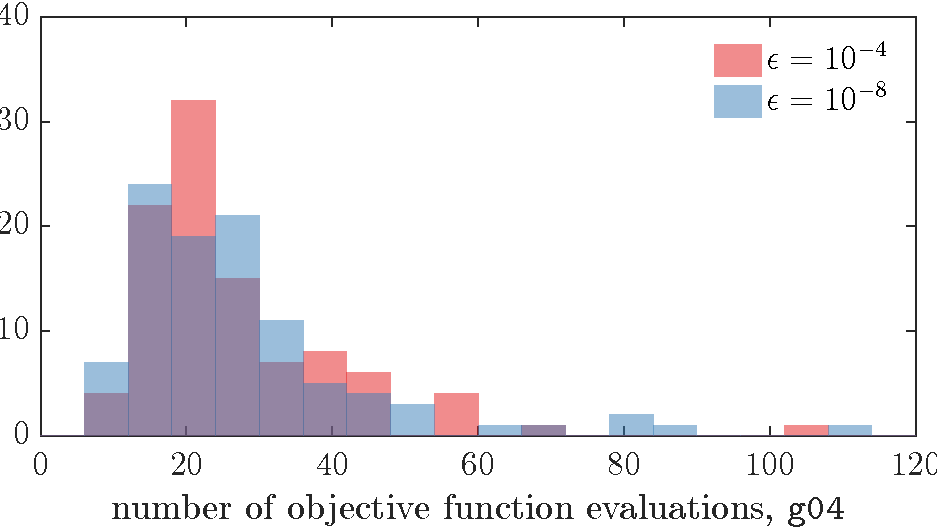
\includegraphics[width=.48\linewidth]{figures/hist04}
    \hfill
    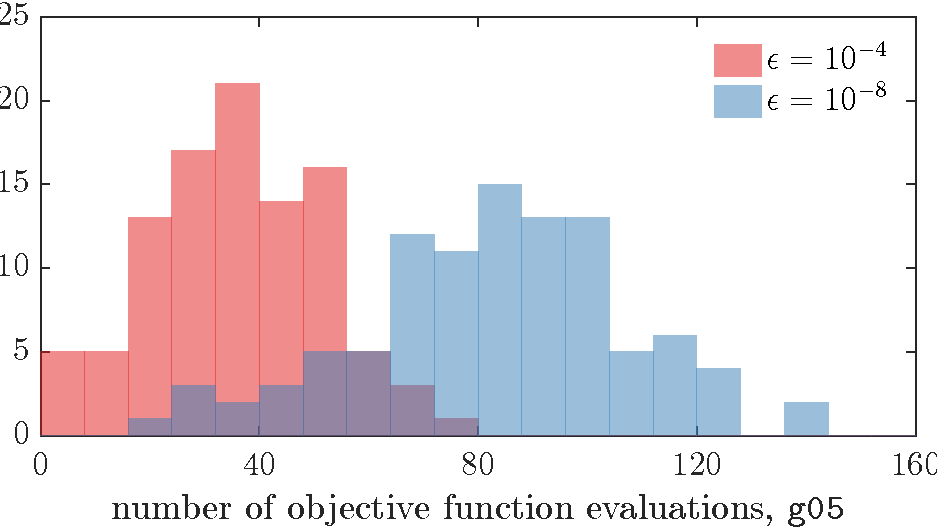
\includegraphics[width=.48\linewidth]{figures/hist05}
    
    \vspace{3.6mm}
    
    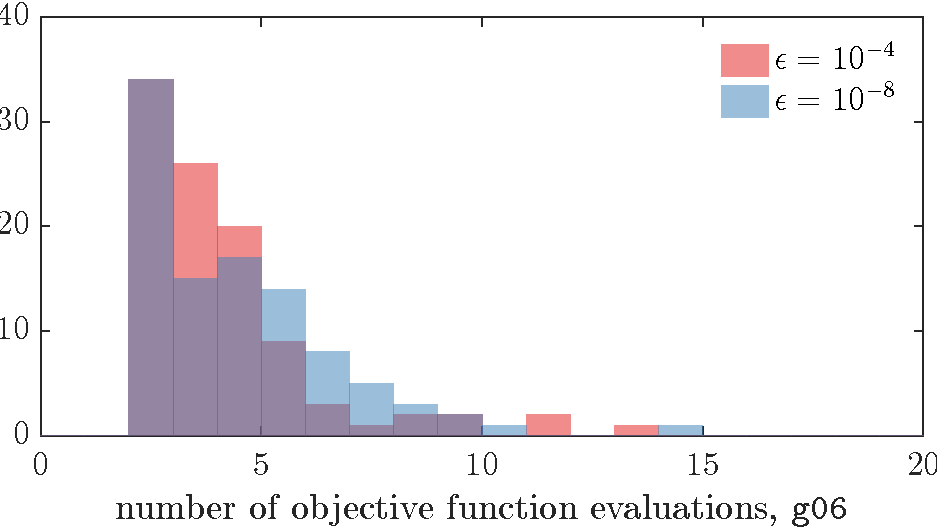
\includegraphics[width=.48\linewidth]{figures/hist06}
    \hfill
    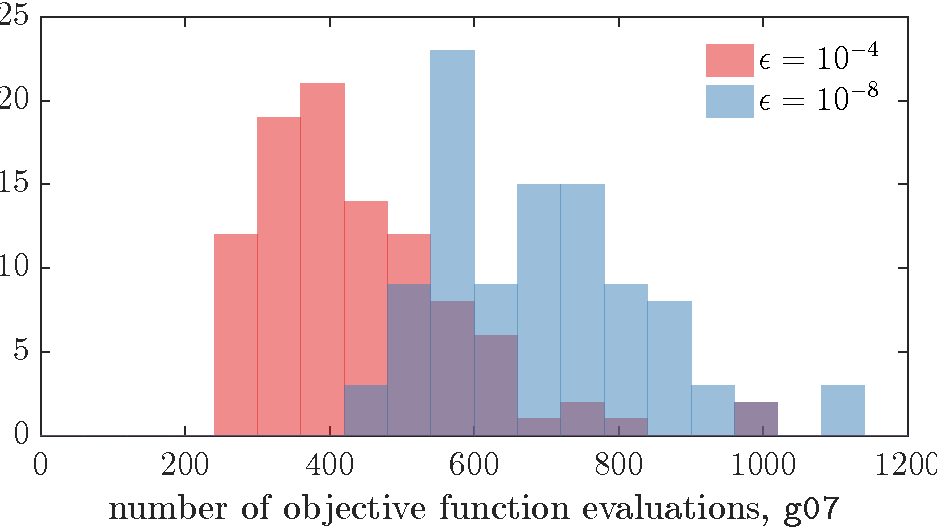
\includegraphics[width=.48\linewidth]{figures/hist07}

    \vspace{3.6mm}
    
    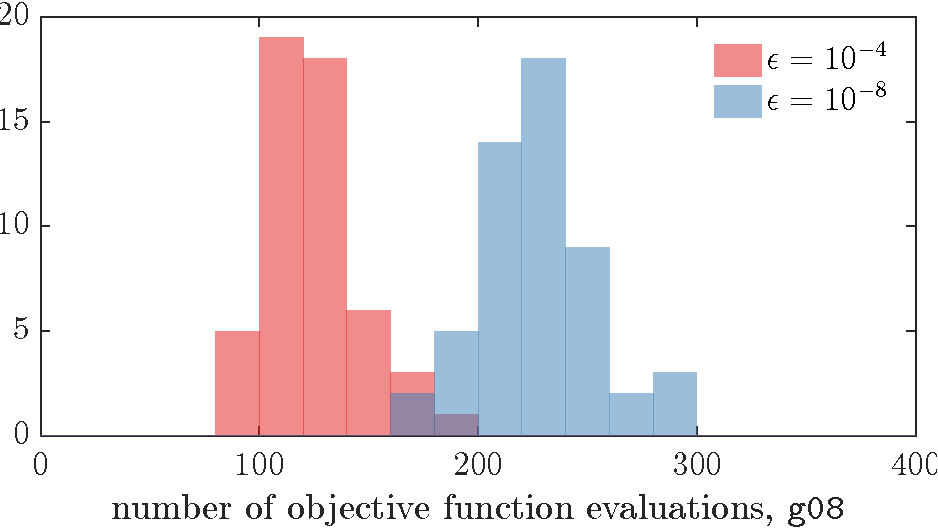
\includegraphics[width=.48\linewidth]{figures/hist08}
    \hfill
    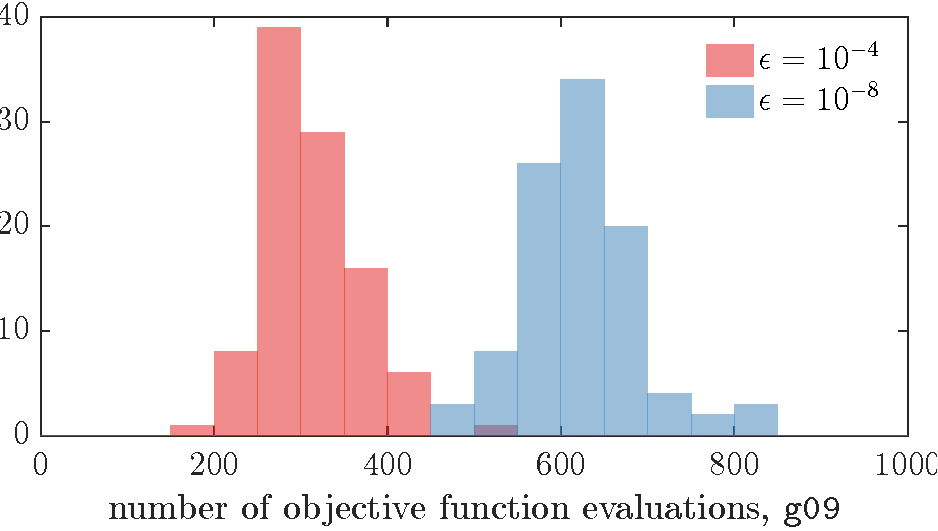
\includegraphics[width=.48\linewidth]{figures/hist09}
    
    \vspace{3.6mm}
    
    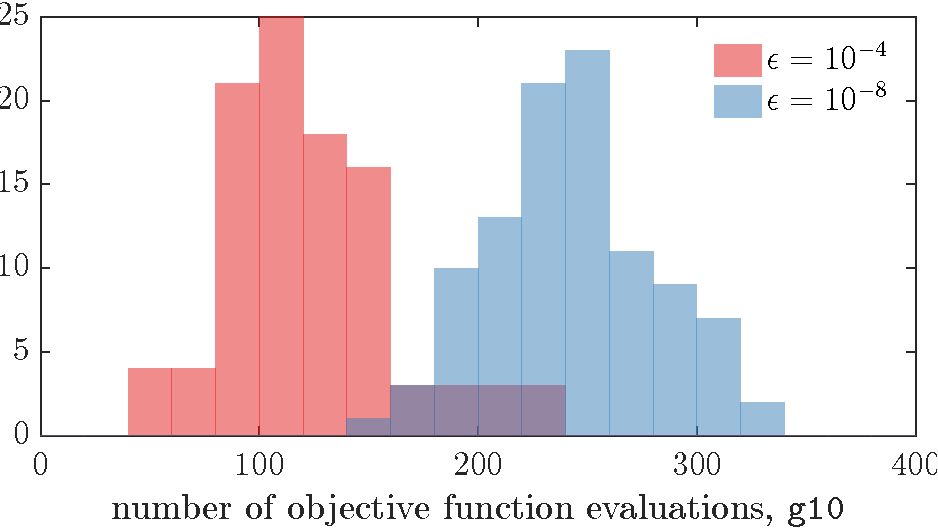
\includegraphics[width=.48\linewidth]{figures/hist10}
    \hfill
    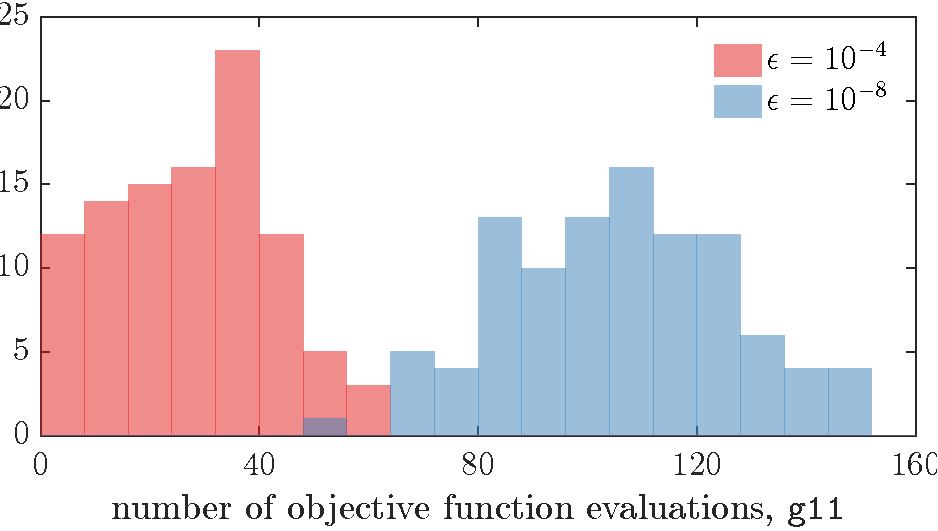
\includegraphics[width=.48\linewidth]{figures/hist11}      
  \end{minipage}
  \caption{\label{fig.histograms}Histograms showing the number of objective function evaluations required to solve problems \texttt{g01} and \texttt{g03} through \texttt{g11}.}
\end{figure}

Figure~\ref{fig.histograms} shows histograms of the number of objective function evaluations required to solve problems \texttt{g01} and \texttt{g03} through \texttt{g11} to both target accuracies. The ranges of the histograms are such that all successful runs are included.  No data are shown for \texttt{g02} as no successful runs were observed for that problem. It can be seen that the histograms for \texttt{g01}, \texttt{g04}, and \texttt{g06} differ fundamentally from those for the other problems in that there is little difference between the data for $\epsilon=10^{-4}$ and $\epsilon=10^{-8}$. This is due to the dimension of the optimal reduced search space being zero. In that case, solving for the solution at the intersection of the active constraints yields the optimal solution (up to the limits of numerical accuracy). For the remaining problems, the gap between the histograms for $\epsilon=10^{-4}$ and $\epsilon=10^{-8}$ is due to the need for the $(1+1)$-ES to search a non-zero reduced search space, with a larger discrepancy for those cases where the dimension of that space is large.
  
\begin{figure}
  \begin{minipage}{\linewidth}
    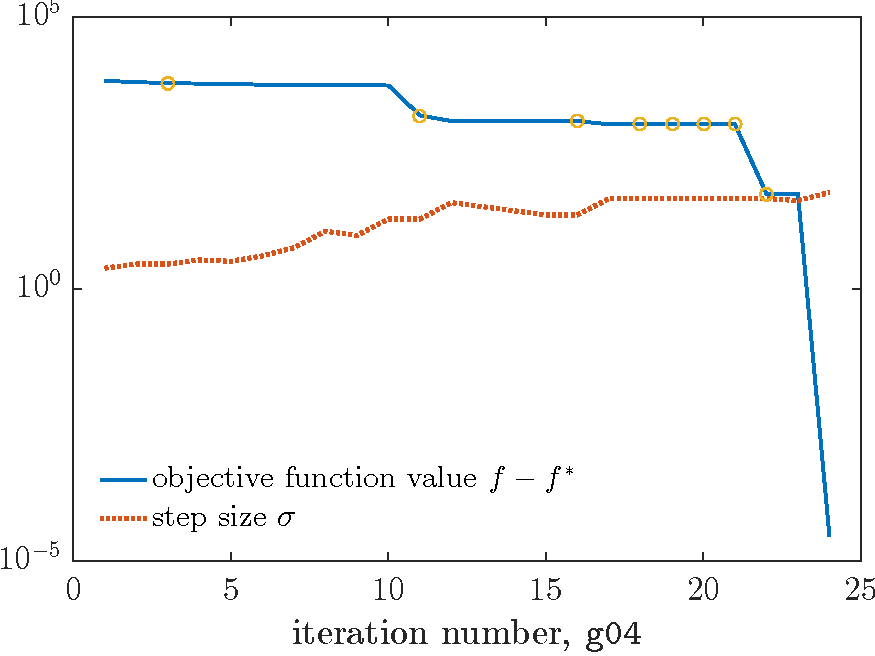
\includegraphics[width=.48\linewidth]{figures/medianRun04}
    \hfill
    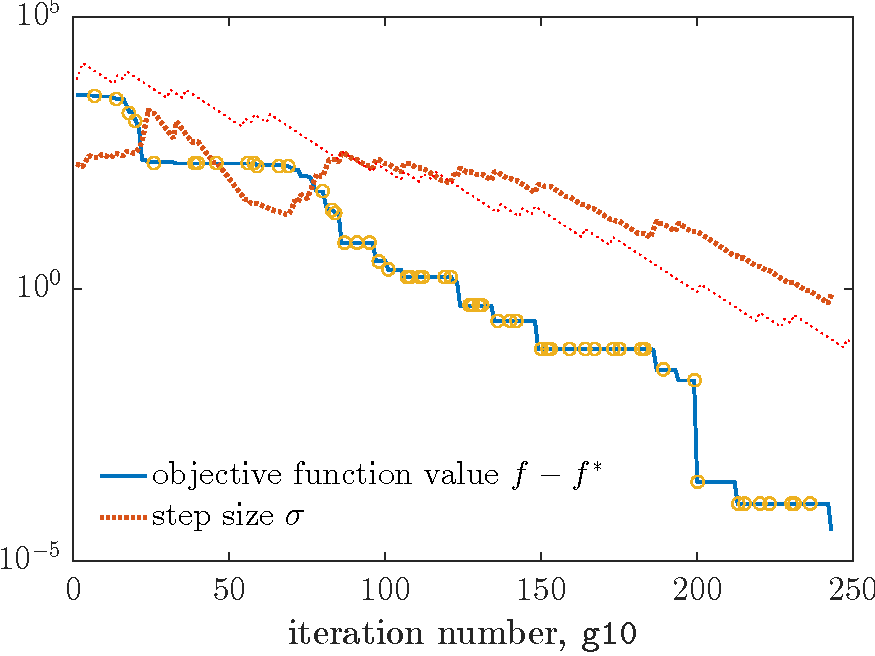
\includegraphics[width=.48\linewidth]{figures/medianRun10}
  \end{minipage}
  \caption{\label{fig.sampleruns}Traces from runs requiring the median number
    of iterations to reach target accuracy $\epsilon=10^{-8}$ for problems
    \texttt{g04} and \texttt{g10}. The evolution of both the difference
    between $f(\x)$ and the optimal objective function value $f^*$ and the
    step size $\sigma$ are shown. The small circles mark those iterations
    where the use of the active set is suspended. The thin dotted line in the
    plot for \texttt{g10} shows the evolution of the step size in a typical
    run of the $(1+1)$-ES on an unconstrained, two-dimensional sphere
    function.}
\end{figure}

Figure~\ref{fig.sampleruns} shows traces from runs requiring the median number of iterations to reach target accuracy $\epsilon=10^{-8}$ for test problems \texttt{g04} and \texttt{g10}. The former is an example of a problem where the dimension of the optimal reduced search space is zero; for the latter, that dimension is $n^*=2$. Plotted against the iteration number are the difference between the objective function value $f(\x)$ and the optimal objective function value $f^*$ as well as the step size $\sigma$ of the algorithm. Those iterations where the algorithm suspends the use of the active set (i.e., $\kappa$ is true) are marked with small circles.

In the run on \texttt{g04}, the evolution strategy generates the optimal active set~$\mathcal{A}^*$ in iteration~24, at which point it terminates. Between iterations 18 and 21, the use of the active set is suspended in each step as it is such that the dimension of the reduced search space is zero. The step size~$\sigma$ largely increases through most of the run.

In the run on \texttt{g10}, the algorithm arrives at the optimal active set~$\mathcal{A}^*$, which consists of the six constraints active at the global optimum of the problem, at iteration~70. The active set remains stable after this, and optimization effectively proceeds in a reduced subspace of dimension $n^*=2$, with the exception of those steps where the use of the active set is suspended, but which have no further effect on the sequence of successful candidate solution generated. It can be seen that the step size~$\sigma$ largely decreases as the search in the two-dimensional subspace progresses. Comparison with the thin dotted curve, which shows the rate of decrease of the step size of a $(1+1)$-ES on an unconstrained, two-dimensional sphere function, shows a similar rate of linear convergence.

A comparison of the performance of the active-set $(1+1)$-ES with that of other approaches to constrained evolutionary optimization is not straightforward as both initialization conditions and termination criteria often differ for approaches found in the literature. More significantly, most other approaches consider the constraint functions as black boxes and are thus not easily able to project candidate solutions onto the feasible region (or subspaces thereof). That said, some useful points of comparison do exist:
\begin{itemize}
  \item The numbers of objective function evaluations required by the active covariance matrix adaptation based approach by Arnold and Hansen~\cite{arnold12a} to solve four of the problems\footnote{Multimodal problems and those with equality constraints were not considered in that paper, leaving only problems \texttt{g06}, \texttt{g07}, \texttt{g09}, and \texttt{g10}.} to target accuracy $10^{-8}$ range from 308 for \texttt{g06} to 3,{}976 for \texttt{g10}. The corresponding figures from Table~\ref{tab.results} range from 4 for \texttt{g06} to 684 for \texttt{g07}. It is important to keep in mind though that the active-set approach introduced here assumes knowledge of the constraint functions, whereas the algorithm from~\cite{arnold12a} considers the constraint functions as black boxes. 
  \item The algorithm by Takahama and Sakai~\cite{TS06}, which performed best among all entries submitted to the \textsl{CEC 2006 Special Session on Constrained Real-Parameter Optimization}, assumes knowledge of gradient vectors and thus does not treat the constraint functions as black boxes. It requires median numbers of objective function evaluations ranging from 1,{}182 for \texttt{g08} to 105,{}799 for \texttt{g10}. The algorithm does successfully solve \texttt{g02}.
%  \item Datta and Deb~\cite{datta15} propose a bi-objective approach that uses \texttt{fmincon} for solving penalized versions of the objective assuming known bound constraints. Median numbers of objective function evaluations required to reach their termination criterion range from 1,{}226 for \texttt{g08} to 49,{}102 for \texttt{g10}. Problem \texttt{g02} is solved, albeit with an even larger number of function evaluations.
  \item Bagheri et al.~\cite{bagheri15} propose SACOBRA, a self-adaptive variant of the surrogate based COBRA algorithm by Regis~\cite{regis14}, which solves most of the eleven problems (though not \texttt{g02}, and others only with limited accuracy) with fewer than 500 objective function evaluations. SACOBRA considers the constraint functions as black boxes and is thus applicable when the constraints are not known. It requires more function evaluations than the active-set $(1+1)$-ES for a number of those problems where the dimension of the optimal reduced search space is low. However, it appears to often converge faster where that dimension is not very small. This latter advantage is a consequence of the smooth nature of the test problems, which admit polynomial surrogate models that make it possible to converge superlinearly. As shown by Teytaud and Gelly~\cite{TG06}, as a comparison-based algorithm that does not use objective function values other than in comparisons, the active-set $(1+1)$-ES cannot exhibit super-linear convergence.
\end{itemize}


\section{\label{sec4}Conclusions}

To conclude, we have proposed an active-set $(1+1)$-ES for constrained numerical optimization with known constraints. The algorithm usually generates offspring candidate solutions constrained to the reduced subspace at their parents, but with a fixed probability samples offspring that do not necessarily fall into that space, thus allowing it to render active constraints inactive. Key to the functioning of the algorithm is to adapt the step size only in those iterations where the offspring are constrained to the reduced search space. The algorithm can be implemented in a few lines of \textsl{Matlab} code and performs very well when compared with related work.

It is of interest to apply the proposed active-set approach in evolutionary algorithms other than the $(1+1)$-ES. The $(\mu/\mu,\lambda)$-ES is an evolutionary algorithm less sensitive to noise and ruggedness of the objective than the $(1+1)$-ES as it is capable of proceeding with larger steps. Restart variants of that algorithm~\cite{auger05} are commonly used for multimodal optimization problems and may exhibit improved performance for problems \texttt{g02} and \texttt{g08}. However, using the active-set approach with cumulative step size adaptation is less than straightforward, and it has been seen that care has to be taken when integrating constraint handling techniques with step size adaptation~\cite{arnold13a,hellwig16}. Also of interest is the problem of employing the active-set approach in combination with other constraint handling techniques, such as augmented Lagrangian methods~\cite{arnold15a}, in case only a proper subset of the constraints is known explicitly. Finally, it is of interest to employ the active-set approach in evolutionary algorithms that use surrogate models of the objective function in order to reduce the time spent on optimization in reduced search spaces.


\subsection*{Acknowledgements}

This research was supported by the Natural Sciences and Engineering Research Council of Canada (NSERC).


\bibliographystyle{plain}
\bibliography{main}

\end{document}
